% !TeX root = 00_Vorlage.tex
% !TeX spellcheck = de_DE

\chapter{Aufbau und Methoden}
\label{sec:aufbau}
In diesem Kapitel wird der Aufbau der drei Einzelversuche erläutert.
\section{Eine Feder mit drei Massen}
Für diesen Versuch wird eine Feder mit jeweils drei verschiedenen Massen $m_i$ in Schwingung versetzt, um aus der Winkelfrequenz die Federkonstante $k$ zu berechnen. Um drei verschiedene Massen zu erhalten, wird der Versuch einmal nur mit dem IOLab durchgeführt. Für den zweiten Durchgang wird ein Stein mit Klebeband an dem IOLab befestigt und für den dritten Durchgang ein weiterer Stein. Ebenfalls benötigt man eine Feder, das IOLab an dem eine Ringschraube an dem Kraftsensor angebracht ist und eine Briefklammer, welche an einer Stuhllehne befestigt ist.
\subsection{Bestimmung der Masse}
Um nun die einzelnen Massen $m_i$ zu bestimmen wird das IOLab an dem Kraftsensor mit einer Schnur, über einen Fixpunkt hochgezogen. (Siehe \autoref{fig:Massenbestimmung}). Dies wird nun für die zwei weiteren Massen wiederholt. Aus den Daten des Beschleunigungs- und Kraftsensors lässt sich die jeweilige Masse bestimmen. 
\begin{figure}[H]
	\centering
	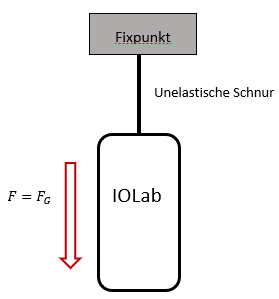
\includegraphics[scale=0.4]{Massebestimmung}
	\caption[Versuchsaufbau der Massebestimmung]{Schematischer Versuchsaufbau zur Bestimmung der Masse}
	\label{fig:Massenbestimmung}
\end{figure}
\subsection{Bestimmung der Winkelfrequenz}
Nun wird die unelastische Schnur durch eine Feder ersetzt und das IOLab wird aus dem Ruhepunkt ausgelenkt. Währenddessen wird die Kraft $F$ die auf den Kraftsensor wirkt und die Beschleunigung $a$ aufgezeichnet. Man erhält einen Sinus-artigen Verlauf in beiden Messungen, aus welchen man die Kreisfrequenz mit einem Sinus-Fit bestimmen kann.
\begin{figure}[H]
	\centering
	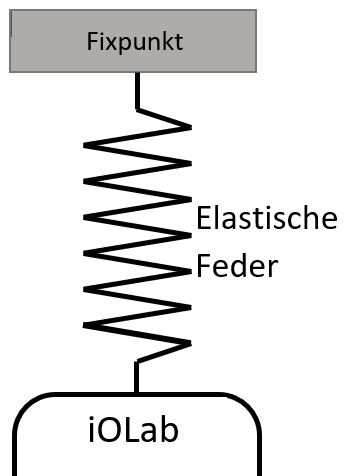
\includegraphics[width=5cm,keepaspectratio]{Schwingung 1}
	\caption[Versuchsaufbau für eine Feder]{Schematische Darstellung des Versuchsaufbau zur Bestimmung der Kreisfrequenz}
	\label{fig:Schwingungsperiode1}
\end{figure}
\subsection{Berechnung der Federkonstante \( k \)}
Wie in \autoref{sec:theorie} diskutiert lässt sich nun der Wert für $k$ durch die Kreisfrequenz und der Masse $m_i$ bestimmen.
\section{Aufstellen eines Modells für parallele Federn}
\label{sec:Modell}
Zur Bestimmung eines Modells für die Gesamtfederkonstante $k_{\text{ges}}$ wird der Versuch mit der schwersten  Masse $m_3$ und zwei parallelen Federn wiederholt. Dazu werden mit Hilfe von zwei Kartonstücken die Federn parallel aufgehängt. Die Kartonstücke werden mit einer Büroklammer an dem Kraftsensor und dem Fixpunkt befestigt, wie \autoref{fig:2,3 Federn} zeigt. Anschließend wird das IOLab aus dem Ruhepunkt ausgelenkt und für $20s$ die Kraft $F$ und die Beschleunigung $a$ aufgezeichnet.
\begin{figure}[H]
	\centering
	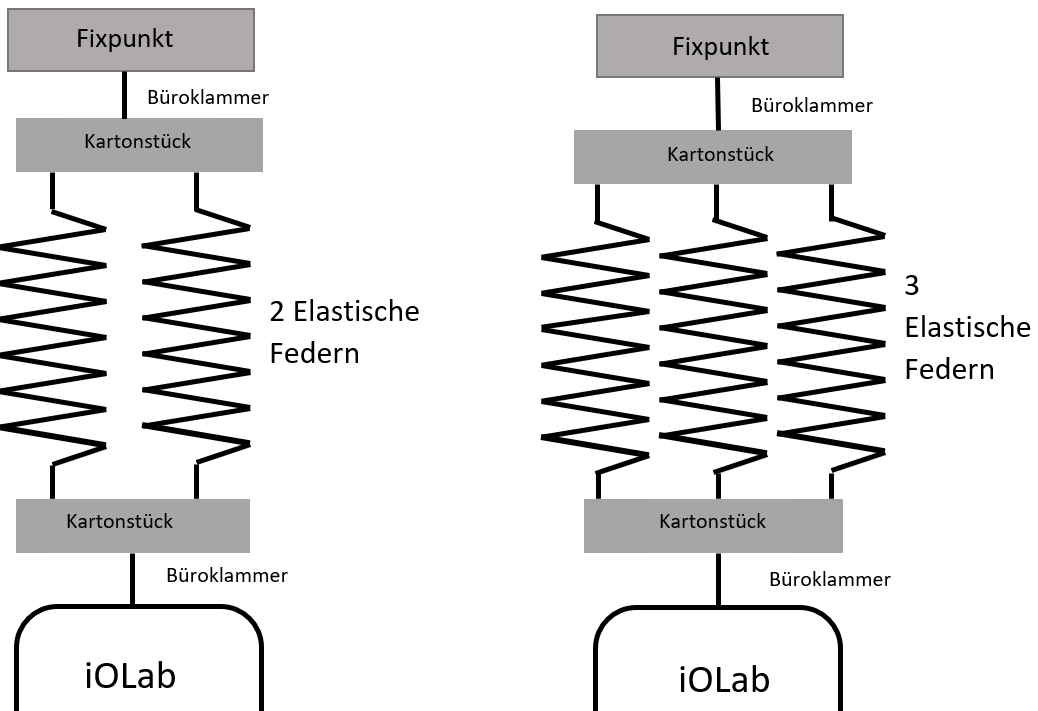
\includegraphics[width=10cm, keepaspectratio]{2,3Federn}
	\caption[Versuchsaufbau mit mehreren Federn]{Schematischer Versuchsaufbau von zwei parallelen Federn(links) und drei Federn (rechts), zur Bestimmung der Periodendauer}
	\label{fig:2,3 Federn}
\end{figure}
Aus dem Vergleich der Federkonstanten $k_1$ und $k_2$ aus \autoref{sec:Modell} lässt sich nun ein Modell für $N$ Federn aufstellen.
\section{Prüfen des Modells}
Um nun das Modell zu überprüfen, erweitern wir obigen Versuch auf drei parallelen Federn mit selbiger Masse $m_3$ (Siehe \autoref{fig:2,3 Federn}). Bei der Durchführung dieses Versuches muss auf die anfängliche Auslenkung geachtet werden, da es zu Überdehnung der Federn kommen kann und das System dann nicht mehr durch einen harmonischen Oszillator beschrieben wird. Anschließend wird wie im vorherigen Versuch die Federkonstante \( k_3 \) ausgerechnet und mit dem Modell abgeglichen.